\subsection{Controller design} \label{PID}
There are one specific controller that is related to this project, the PID (Proportional, Integral, Derivative) controller. This PID controller is used to delimit the errors inside a loop. Each of these Components driving the error to zero, which can be read about in the sections to come. Every component has its own allocated gain, a gain is the ratio between the output divide by the input. The objective in this system is to move from one angle to another, the error would then be difference in angles over time. In this section \textbf{\textit{U}} is denoted as being the effort to be put in the system.\\

\begin{figure}
    \centering
    

\tikzset{every picture/.style={line width=0.75pt}} %set default line width to 0.75pt        

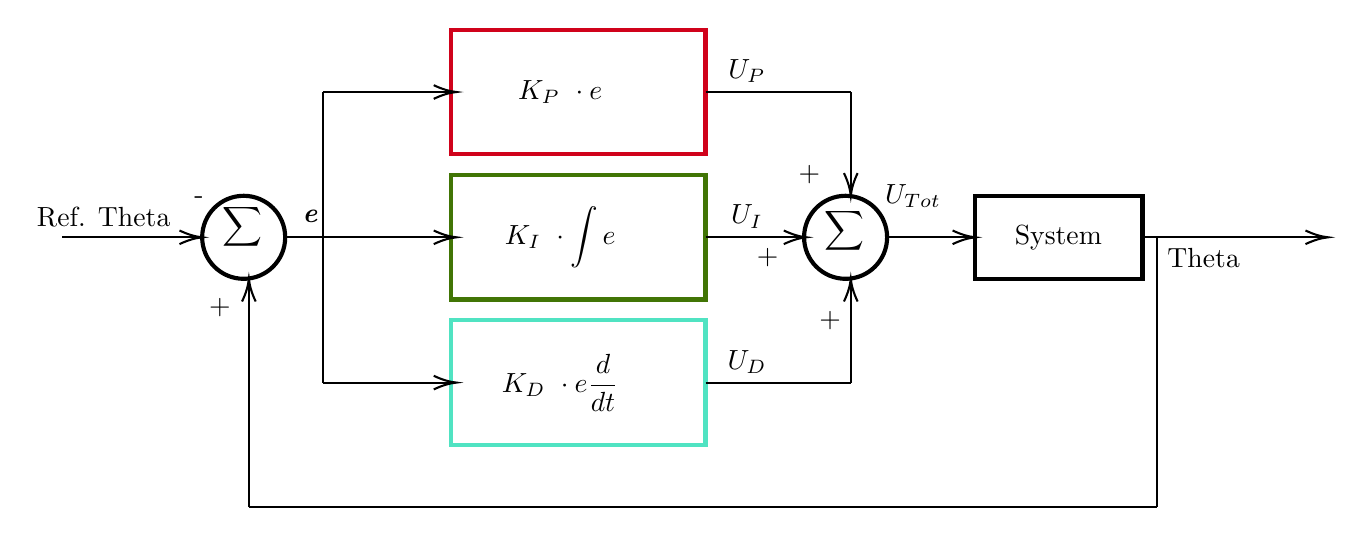
\begin{tikzpicture}[x=0.75pt,y=0.75pt,yscale=-1,xscale=1]
%uncomment if require: \path (0,269); %set diagram left start at 0, and has height of 269

%Shape: Rectangle [id:dp6186698400269734] 
\draw  [color={rgb, 255:red, 208; green, 2; blue, 27 }  ,draw opacity=1 ][line width=1.5]  (217.5,20) -- (340,20) -- (340,80) -- (217.5,80) -- cycle ;
%Shape: Rectangle [id:dp35497397654468] 
\draw  [color={rgb, 255:red, 65; green, 117; blue, 5 }  ,draw opacity=1 ][line width=1.5]  (217.5,90) -- (340,90) -- (340,150) -- (217.5,150) -- cycle ;
%Shape: Rectangle [id:dp0011241398633399236] 
\draw  [color={rgb, 255:red, 80; green, 227; blue, 194 }  ,draw opacity=1 ][line width=1.5]  (217.5,160) -- (340,160) -- (340,220) -- (217.5,220) -- cycle ;
%Shape: Circle [id:dp7081049529214984] 
\draw  [line width=1.5]  (97.5,120) .. controls (97.5,108.95) and (106.45,100) .. (117.5,100) .. controls (128.55,100) and (137.5,108.95) .. (137.5,120) .. controls (137.5,131.05) and (128.55,140) .. (117.5,140) .. controls (106.45,140) and (97.5,131.05) .. (97.5,120) -- cycle ;
%Straight Lines [id:da1012548517194285] 
\draw    (155.61,50) -- (218,50) ;
\draw [shift={(220,50)}, rotate = 180] [color={rgb, 255:red, 0; green, 0; blue, 0 }  ][line width=0.75]    (10.93,-3.29) .. controls (6.95,-1.4) and (3.31,-0.3) .. (0,0) .. controls (3.31,0.3) and (6.95,1.4) .. (10.93,3.29)   ;

%Straight Lines [id:da024552935574742696] 
\draw    (137.5,120) -- (218,120) ;
\draw [shift={(220,120)}, rotate = 180] [color={rgb, 255:red, 0; green, 0; blue, 0 }  ][line width=0.75]    (10.93,-3.29) .. controls (6.95,-1.4) and (3.31,-0.3) .. (0,0) .. controls (3.31,0.3) and (6.95,1.4) .. (10.93,3.29)   ;

%Straight Lines [id:da632489535879416] 
\draw    (155.61,190) -- (218,190) ;
\draw [shift={(220,190)}, rotate = 180] [color={rgb, 255:red, 0; green, 0; blue, 0 }  ][line width=0.75]    (10.93,-3.29) .. controls (6.95,-1.4) and (3.31,-0.3) .. (0,0) .. controls (3.31,0.3) and (6.95,1.4) .. (10.93,3.29)   ;

%Straight Lines [id:da028164362822356237] 
\draw    (155.61,50) -- (155.61,110) ;


%Straight Lines [id:da1783990189247291] 
\draw    (155.61,110) -- (155.61,190) ;


%Shape: Ellipse [id:dp13776991374733094] 
\draw  [line width=1.5]  (387.5,120) .. controls (387.5,108.95) and (396.45,100) .. (407.5,100) .. controls (418.55,100) and (427.5,108.95) .. (427.5,120) .. controls (427.5,131.05) and (418.55,140) .. (407.5,140) .. controls (396.45,140) and (387.5,131.05) .. (387.5,120) -- cycle ;
%Straight Lines [id:da5590648239872058] 
\draw    (340,50) -- (410,50) ;


%Straight Lines [id:da32339100567036794] 
\draw    (340,120) -- (386.65,120) ;
\draw [shift={(388.65,120)}, rotate = 180] [color={rgb, 255:red, 0; green, 0; blue, 0 }  ][line width=0.75]    (10.93,-3.29) .. controls (6.95,-1.4) and (3.31,-0.3) .. (0,0) .. controls (3.31,0.3) and (6.95,1.4) .. (10.93,3.29)   ;

%Straight Lines [id:da37714274354973676] 
\draw    (340,190) -- (410,190) ;


%Straight Lines [id:da12414839144602552] 
\draw    (410,50) -- (410,98) ;
\draw [shift={(410,100)}, rotate = 270] [color={rgb, 255:red, 0; green, 0; blue, 0 }  ][line width=0.75]    (10.93,-3.29) .. controls (6.95,-1.4) and (3.31,-0.3) .. (0,0) .. controls (3.31,0.3) and (6.95,1.4) .. (10.93,3.29)   ;

%Straight Lines [id:da2294854556231043] 
\draw    (410,142) -- (410,190) ;

\draw [shift={(410,140)}, rotate = 90] [color={rgb, 255:red, 0; green, 0; blue, 0 }  ][line width=0.75]    (10.93,-3.29) .. controls (6.95,-1.4) and (3.31,-0.3) .. (0,0) .. controls (3.31,0.3) and (6.95,1.4) .. (10.93,3.29)   ;
%Straight Lines [id:da7636925489142845] 
\draw    (427.5,120) -- (468,120) ;
\draw [shift={(470,120)}, rotate = 180] [color={rgb, 255:red, 0; green, 0; blue, 0 }  ][line width=0.75]    (10.93,-3.29) .. controls (6.95,-1.4) and (3.31,-0.3) .. (0,0) .. controls (3.31,0.3) and (6.95,1.4) .. (10.93,3.29)   ;

%Straight Lines [id:da8120471221631163] 
\draw    (30,120) -- (95.5,120) ;
\draw [shift={(97.5,120)}, rotate = 180] [color={rgb, 255:red, 0; green, 0; blue, 0 }  ][line width=0.75]    (10.93,-3.29) .. controls (6.95,-1.4) and (3.31,-0.3) .. (0,0) .. controls (3.31,0.3) and (6.95,1.4) .. (10.93,3.29)   ;

%Straight Lines [id:da7263862005723072] 
\draw    (120,250) -- (120,142) ;
\draw [shift={(120,140)}, rotate = 450] [color={rgb, 255:red, 0; green, 0; blue, 0 }  ][line width=0.75]    (10.93,-3.29) .. controls (6.95,-1.4) and (3.31,-0.3) .. (0,0) .. controls (3.31,0.3) and (6.95,1.4) .. (10.93,3.29)   ;

%Straight Lines [id:da9777886662003494] 
\draw    (120,250) -- (490,250) ;


%Shape: Rectangle [id:dp7284343716119925] 
\draw  [line width=1.5]  (470,100) -- (550.53,100) -- (550.53,140) -- (470,140) -- cycle ;
%Straight Lines [id:da4771680795774551] 
\draw    (550.53,120) -- (638,120) ;
\draw [shift={(640,120)}, rotate = 180] [color={rgb, 255:red, 0; green, 0; blue, 0 }  ][line width=0.75]    (10.93,-3.29) .. controls (6.95,-1.4) and (3.31,-0.3) .. (0,0) .. controls (3.31,0.3) and (6.95,1.4) .. (10.93,3.29)   ;

%Straight Lines [id:da7739849283065594] 
\draw    (557.37,120) -- (557.37,250) ;


%Straight Lines [id:da5629774692956326] 
\draw    (557.37,250) -- (485.79,250) ;



% Text Node
\draw (50,110) node  [align=left] {Ref. Theta};
% Text Node
\draw (510,120) node  [align=left] {System};
% Text Node
\draw (270,190) node  [align=left] {$\displaystyle K_{D} \ \cdot e  \frac{d}{dt}$};
% Text Node
\draw (270,120) node  [align=left] {$\displaystyle K_{I} \ \cdot \int e$};
% Text Node
\draw (270,50) node  [align=left] {$\displaystyle K_{P} \ \cdot e$};
% Text Node
\draw (390,90) node  [align=left] {+};
% Text Node
\draw (370,130) node  [align=left] {+};
% Text Node
\draw (400,160) node  [align=left] {+};
% Text Node
\draw (106,154) node  [align=left] {+};
% Text Node
\draw (96,101) node  [align=left] {\mbox{-}};
% Text Node
\draw (150,110) node  [align=left] {\textit{\textbf{e}}};
% Text Node
\draw (407,117) node  [align=left] {$\displaystyle \sum $};
% Text Node
\draw (360,110) node  [align=left] {$\displaystyle U_{I}$};
% Text Node
\draw (360,180) node  [align=left] {$\displaystyle U_{D}$};
% Text Node
\draw (360,40) node  [align=left] {$\displaystyle U_{P}$};
% Text Node
\draw (117,115) node  [align=left] {$\displaystyle \sum $};
% Text Node
\draw (440,100) node  [align=left] {$\displaystyle U_{Tot}$};
% Text Node
\draw (580,130) node  [align=left] {Theta};


\end{tikzpicture}

    %\includegraphics{Figures/Technical_figures/1-25.jpg}
    \caption{Layout of a PID controllers response on the error}
    \label{fig:mPID}
\end{figure}


\begin{equation}\label{PID}
    U=K_P\cdot\textit{e}+K_I\cdot\int\textit{e}+K_D\cdot\textit{e}\frac{d}{dt}
\end{equation}

\paragraph{The Proportional} gain $K_P$ in eq.\ref{PID} is the gain multiplied with the error(e) in eq. \ref{PID}, resulting in the effort. The larger gain a fast rise time, the rise time is the time it takes from 10\% to 90\% of the final angle. However this controller can only be used alone when the system can tolerate a constant error in steady state, a steady state error is an error over time that does not diminish. The proportional gain also has a tendency to overshoot the desired value if the gain is too high\cite{Control1DK}.\\

\begin{figure}[H]
    \centering
    \includegraphics[width=\textwidth]{Figures/Technical_figures/PGAIN.png} 
    %

\tikzset{every picture/.style={line width=0.75pt}} %set default line width to 0.75pt        

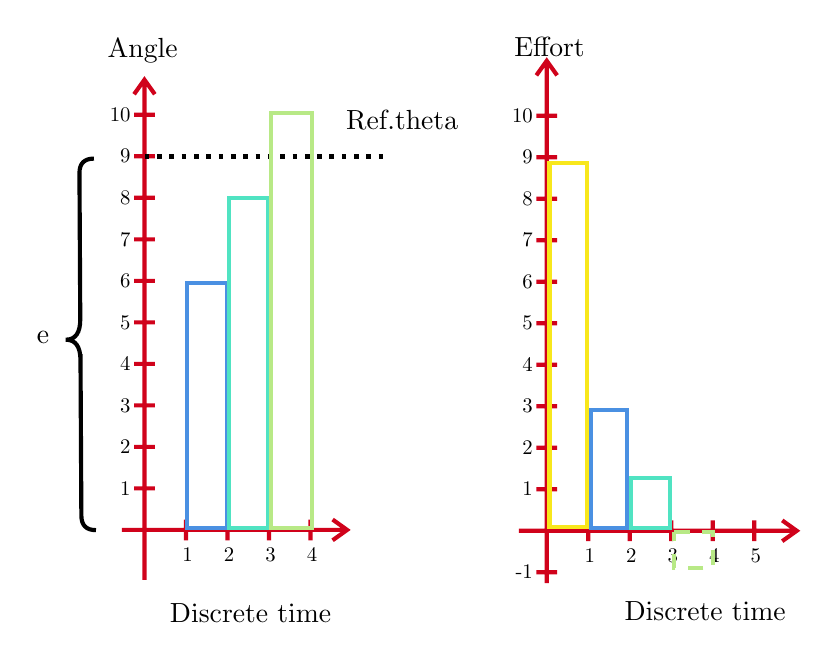
\begin{tikzpicture}[x=0.75pt,y=0.75pt,yscale=-1,xscale=1]
%uncomment if require: \path (0,530); %set diagram left start at 0, and has height of 530

%Shape: Axis 2D [id:dp45682595351826527] 
\draw [color={rgb, 255:red, 208; green, 2; blue, 27 }  ,draw opacity=1 ][line width=1.5]  (90,242.9) -- (198.5,242.9)(100.85,26) -- (100.85,267) (191.5,237.9) -- (198.5,242.9) -- (191.5,247.9) (95.85,33) -- (100.85,26) -- (105.85,33) (120.85,237.9) -- (120.85,247.9)(140.85,237.9) -- (140.85,247.9)(160.85,237.9) -- (160.85,247.9)(180.85,237.9) -- (180.85,247.9)(95.85,222.9) -- (105.85,222.9)(95.85,202.9) -- (105.85,202.9)(95.85,182.9) -- (105.85,182.9)(95.85,162.9) -- (105.85,162.9)(95.85,142.9) -- (105.85,142.9)(95.85,122.9) -- (105.85,122.9)(95.85,102.9) -- (105.85,102.9)(95.85,82.9) -- (105.85,82.9)(95.85,62.9) -- (105.85,62.9)(95.85,42.9) -- (105.85,42.9) ;
\draw   (127.85,254.9) node[anchor=east, scale=0.75]{1} (147.85,254.9) node[anchor=east, scale=0.75]{2} (167.85,254.9) node[anchor=east, scale=0.75]{3} (187.85,254.9) node[anchor=east, scale=0.75]{4} (97.85,222.9) node[anchor=east, scale=0.75]{1} (97.85,202.9) node[anchor=east, scale=0.75]{2} (97.85,182.9) node[anchor=east, scale=0.75]{3} (97.85,162.9) node[anchor=east, scale=0.75]{4} (97.85,142.9) node[anchor=east, scale=0.75]{5} (97.85,122.9) node[anchor=east, scale=0.75]{6} (97.85,102.9) node[anchor=east, scale=0.75]{7} (97.85,82.9) node[anchor=east, scale=0.75]{8} (97.85,62.9) node[anchor=east, scale=0.75]{9} (97.85,42.9) node[anchor=east, scale=0.75]{10} ;
%Straight Lines [id:da07124731425948538] 
\draw [line width=1.5]  [dash pattern={on 1.69pt off 2.76pt}]  (101,63) -- (218.5,63) ;


%Shape: Brace [id:dp5273011604952158] 
\draw  [line width=1.5]  (76.5,64) .. controls (71.83,64.03) and (69.51,66.37) .. (69.54,71.04) -- (69.93,141.23) .. controls (69.97,147.9) and (67.66,151.24) .. (62.99,151.27) .. controls (67.66,151.24) and (70.01,154.56) .. (70.04,161.23)(70.03,158.23) -- (70.46,236.04) .. controls (70.49,240.71) and (72.83,243.03) .. (77.5,243) ;
%Shape: Rectangle [id:dp5387283033097741] 
\draw  [color={rgb, 255:red, 74; green, 144; blue, 226 }  ,draw opacity=1 ][line width=1.5]  (121.5,124) -- (140.5,124) -- (140.5,242) -- (121.5,242) -- cycle ;
%Shape: Rectangle [id:dp6947960238766453] 
\draw  [color={rgb, 255:red, 80; green, 227; blue, 194 }  ,draw opacity=1 ][line width=1.5]  (141.67,83) -- (160.5,83) -- (160.5,242) -- (141.67,242) -- cycle ;
%Shape: Rectangle [id:dp8600292583953892] 
\draw  [color={rgb, 255:red, 184; green, 233; blue, 134 }  ,draw opacity=1 ][line width=1.5]  (161.67,42) -- (181.67,42) -- (181.67,242) -- (161.67,242) -- cycle ;
%Shape: Axis 2D [id:dp2561048365476184] 
\draw [color={rgb, 255:red, 208; green, 2; blue, 27 }  ,draw opacity=1 ][line width=1.5]  (281.28,243.33) -- (415.13,243.33)(294.67,16.89) -- (294.67,268.49) (408.13,238.33) -- (415.13,243.33) -- (408.13,248.33) (289.67,23.89) -- (294.67,16.89) -- (299.67,23.89) (314.67,238.33) -- (314.67,248.33)(334.67,238.33) -- (334.67,248.33)(354.67,238.33) -- (354.67,248.33)(374.67,238.33) -- (374.67,248.33)(394.67,238.33) -- (394.67,248.33)(289.67,223.33) -- (299.67,223.33)(289.67,203.33) -- (299.67,203.33)(289.67,183.33) -- (299.67,183.33)(289.67,163.33) -- (299.67,163.33)(289.67,143.33) -- (299.67,143.33)(289.67,123.33) -- (299.67,123.33)(289.67,103.33) -- (299.67,103.33)(289.67,83.33) -- (299.67,83.33)(289.67,63.33) -- (299.67,63.33)(289.67,43.33) -- (299.67,43.33)(289.67,263.33) -- (299.67,263.33) ;
\draw   (321.67,255.33) node[anchor=east, scale=0.75]{1} (341.67,255.33) node[anchor=east, scale=0.75]{2} (361.67,255.33) node[anchor=east, scale=0.75]{3} (381.67,255.33) node[anchor=east, scale=0.75]{4} (401.67,255.33) node[anchor=east, scale=0.75]{5} (291.67,223.33) node[anchor=east, scale=0.75]{1} (291.67,203.33) node[anchor=east, scale=0.75]{2} (291.67,183.33) node[anchor=east, scale=0.75]{3} (291.67,163.33) node[anchor=east, scale=0.75]{4} (291.67,143.33) node[anchor=east, scale=0.75]{5} (291.67,123.33) node[anchor=east, scale=0.75]{6} (291.67,103.33) node[anchor=east, scale=0.75]{7} (291.67,83.33) node[anchor=east, scale=0.75]{8} (291.67,63.33) node[anchor=east, scale=0.75]{9} (291.67,43.33) node[anchor=east, scale=0.75]{10} (291.67,263.33) node[anchor=east, scale=0.75]{-1} ;
%Shape: Rectangle [id:dp9341644709395209] 
\draw  [color={rgb, 255:red, 248; green, 231; blue, 28 }  ,draw opacity=1 ][line width=1.5]  (296,66) -- (314,66) -- (314,241.33) -- (296,241.33) -- cycle ;
%Shape: Rectangle [id:dp4499585049078272] 
\draw  [color={rgb, 255:red, 74; green, 144; blue, 226 }  ,draw opacity=1 ][line width=1.5]  (315.83,185) -- (333.33,185) -- (333.33,242) -- (315.83,242) -- cycle ;
%Shape: Rectangle [id:dp5245979736475872] 
\draw  [color={rgb, 255:red, 80; green, 227; blue, 194 }  ,draw opacity=1 ][line width=1.5]  (335.33,218) -- (354,218) -- (354,242) -- (335.33,242) -- cycle ;
%Shape: Rectangle [id:dp4864189057319952] 
\draw  [color={rgb, 255:red, 184; green, 233; blue, 134 }  ,draw opacity=1 ][dash pattern={on 5.63pt off 4.5pt}][line width=1.5]  (356,244) -- (374.67,244) -- (374.67,261.33) -- (356,261.33) -- cycle ;

% Text Node
\draw (225,45.33) node  [align=left] {Ref.theta};
% Text Node
\draw (52,150) node  [align=left] {e};
% Text Node
\draw (100,12) node  [align=left] {Angle};
% Text Node
\draw (152,283) node  [align=left] {Discrete time};
% Text Node
\draw (296,10) node  [align=left] {Effort};
% Text Node
\draw (371,282) node  [align=left] {Discrete time};


\end{tikzpicture}

    \caption{A $K_P$ of 1 then only the error has and effect on the effort}
    \label{fig:pGain}
\end{figure}

\paragraph{The Integral} gain $K_I$ in eq. \ref{PID} of the controller, accumulates error over time to output an effort to be put in the system. This means that it has a damping effect on the system. This Integral component can be used to minimise overshoot and eliminated the steady state error, that is in the p gain alone. This system accomplish this at the cost of a slow rise time. Thereby being slower to reach its desired destination than with a P gain alone, but will reach there in time. As safety is important when working with people this system would be very suited. However as this is a slow system the precision should be weighed against speed\cite{Control1DK}. \\

\begin{figure}[H]
    \centering
    \includegraphics[width=\textwidth]{Figures/Technical_figures/IGAIN.png} 
    %

\tikzset{every picture/.style={line width=0.75pt}} %set default line width to 0.75pt        

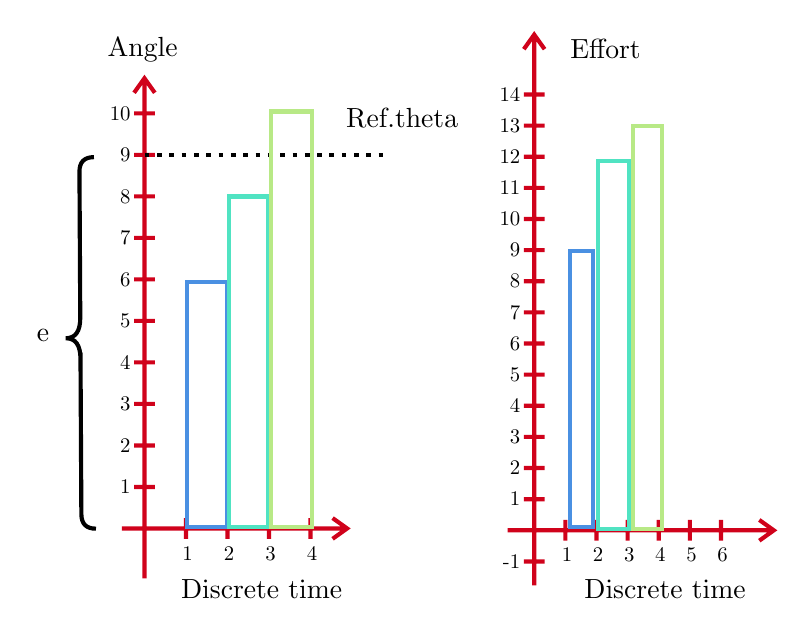
\begin{tikzpicture}[x=0.75pt,y=0.75pt,yscale=-1,xscale=1]
%uncomment if require: \path (0,530); %set diagram left start at 0, and has height of 530

%Shape: Axis 2D [id:dp6346571706526563] 
\draw [color={rgb, 255:red, 208; green, 2; blue, 27 }  ,draw opacity=1 ][line width=1.5]  (86,259.9) -- (194.5,259.9)(96.85,43) -- (96.85,284) (187.5,254.9) -- (194.5,259.9) -- (187.5,264.9) (91.85,50) -- (96.85,43) -- (101.85,50) (116.85,254.9) -- (116.85,264.9)(136.85,254.9) -- (136.85,264.9)(156.85,254.9) -- (156.85,264.9)(176.85,254.9) -- (176.85,264.9)(91.85,239.9) -- (101.85,239.9)(91.85,219.9) -- (101.85,219.9)(91.85,199.9) -- (101.85,199.9)(91.85,179.9) -- (101.85,179.9)(91.85,159.9) -- (101.85,159.9)(91.85,139.9) -- (101.85,139.9)(91.85,119.9) -- (101.85,119.9)(91.85,99.9) -- (101.85,99.9)(91.85,79.9) -- (101.85,79.9)(91.85,59.9) -- (101.85,59.9) ;
\draw   (123.85,271.9) node[anchor=east, scale=0.75]{1} (143.85,271.9) node[anchor=east, scale=0.75]{2} (163.85,271.9) node[anchor=east, scale=0.75]{3} (183.85,271.9) node[anchor=east, scale=0.75]{4} (93.85,239.9) node[anchor=east, scale=0.75]{1} (93.85,219.9) node[anchor=east, scale=0.75]{2} (93.85,199.9) node[anchor=east, scale=0.75]{3} (93.85,179.9) node[anchor=east, scale=0.75]{4} (93.85,159.9) node[anchor=east, scale=0.75]{5} (93.85,139.9) node[anchor=east, scale=0.75]{6} (93.85,119.9) node[anchor=east, scale=0.75]{7} (93.85,99.9) node[anchor=east, scale=0.75]{8} (93.85,79.9) node[anchor=east, scale=0.75]{9} (93.85,59.9) node[anchor=east, scale=0.75]{10} ;
%Straight Lines [id:da8395435041805068] 
\draw [line width=1.5]  [dash pattern={on 1.69pt off 2.76pt}]  (97,80) -- (214.5,80) ;


%Shape: Brace [id:dp15804314182279944] 
\draw  [line width=1.5]  (72.5,81) .. controls (67.83,81.03) and (65.51,83.37) .. (65.54,88.04) -- (65.93,158.23) .. controls (65.97,164.9) and (63.66,168.24) .. (58.99,168.27) .. controls (63.66,168.24) and (66.01,171.56) .. (66.04,178.23)(66.03,175.23) -- (66.46,253.04) .. controls (66.49,257.71) and (68.83,260.03) .. (73.5,260) ;
%Shape: Rectangle [id:dp5191693992255162] 
\draw  [color={rgb, 255:red, 74; green, 144; blue, 226 }  ,draw opacity=1 ][line width=1.5]  (117.5,141) -- (136.5,141) -- (136.5,259) -- (117.5,259) -- cycle ;
%Shape: Rectangle [id:dp2287664558829514] 
\draw  [color={rgb, 255:red, 80; green, 227; blue, 194 }  ,draw opacity=1 ][line width=1.5]  (137.67,100) -- (156.5,100) -- (156.5,259) -- (137.67,259) -- cycle ;
%Shape: Rectangle [id:dp3261576138135398] 
\draw  [color={rgb, 255:red, 184; green, 233; blue, 134 }  ,draw opacity=1 ][line width=1.5]  (157.67,59) -- (177.67,59) -- (177.67,259) -- (157.67,259) -- cycle ;
%Shape: Axis 2D [id:dp473563119637739] 
\draw [color={rgb, 255:red, 208; green, 2; blue, 27 }  ,draw opacity=1 ][line width=1.5]  (271.82,260.8) -- (400.08,260.8)(284.64,22) -- (284.64,287.33) (393.08,255.8) -- (400.08,260.8) -- (393.08,265.8) (279.64,29) -- (284.64,22) -- (289.64,29) (299.64,255.8) -- (299.64,265.8)(314.64,255.8) -- (314.64,265.8)(329.64,255.8) -- (329.64,265.8)(344.64,255.8) -- (344.64,265.8)(359.64,255.8) -- (359.64,265.8)(374.64,255.8) -- (374.64,265.8)(279.64,245.8) -- (289.64,245.8)(279.64,230.8) -- (289.64,230.8)(279.64,215.8) -- (289.64,215.8)(279.64,200.8) -- (289.64,200.8)(279.64,185.8) -- (289.64,185.8)(279.64,170.8) -- (289.64,170.8)(279.64,155.8) -- (289.64,155.8)(279.64,140.8) -- (289.64,140.8)(279.64,125.8) -- (289.64,125.8)(279.64,110.8) -- (289.64,110.8)(279.64,95.8) -- (289.64,95.8)(279.64,80.8) -- (289.64,80.8)(279.64,65.8) -- (289.64,65.8)(279.64,50.8) -- (289.64,50.8)(279.64,275.8) -- (289.64,275.8) ;
\draw   (306.64,272.8) node[anchor=east, scale=0.75]{1} (321.64,272.8) node[anchor=east, scale=0.75]{2} (336.64,272.8) node[anchor=east, scale=0.75]{3} (351.64,272.8) node[anchor=east, scale=0.75]{4} (366.64,272.8) node[anchor=east, scale=0.75]{5} (381.64,272.8) node[anchor=east, scale=0.75]{6} (281.64,245.8) node[anchor=east, scale=0.75]{1} (281.64,230.8) node[anchor=east, scale=0.75]{2} (281.64,215.8) node[anchor=east, scale=0.75]{3} (281.64,200.8) node[anchor=east, scale=0.75]{4} (281.64,185.8) node[anchor=east, scale=0.75]{5} (281.64,170.8) node[anchor=east, scale=0.75]{6} (281.64,155.8) node[anchor=east, scale=0.75]{7} (281.64,140.8) node[anchor=east, scale=0.75]{8} (281.64,125.8) node[anchor=east, scale=0.75]{9} (281.64,110.8) node[anchor=east, scale=0.75]{10} (281.64,95.8) node[anchor=east, scale=0.75]{11} (281.64,80.8) node[anchor=east, scale=0.75]{12} (281.64,65.8) node[anchor=east, scale=0.75]{13} (281.64,50.8) node[anchor=east, scale=0.75]{14} (281.64,275.8) node[anchor=east, scale=0.75]{-1} ;
%Shape: Rectangle [id:dp06820965849131166] 
\draw  [color={rgb, 255:red, 74; green, 144; blue, 226 }  ,draw opacity=1 ][line width=1.5]  (301.75,126.33) -- (313.08,126.33) -- (313.08,259) -- (301.75,259) -- cycle ;
%Shape: Rectangle [id:dp16997023555555235] 
\draw  [color={rgb, 255:red, 80; green, 227; blue, 194 }  ,draw opacity=1 ][line width=1.5]  (315.5,82.67) -- (330.5,82.67) -- (330.5,260) -- (315.5,260) -- cycle ;
%Shape: Rectangle [id:dp21980087841289575] 
\draw  [color={rgb, 255:red, 184; green, 233; blue, 134 }  ,draw opacity=1 ][line width=1.5]  (332.08,66) -- (346.08,66) -- (346.08,260) -- (332.08,260) -- cycle ;

% Text Node
\draw (221,62.33) node  [align=left] {Ref.theta};
% Text Node
\draw (48,167) node  [align=left] {e};
% Text Node
\draw (96,29) node  [align=left] {Angle};
% Text Node
\draw (153.33,289) node  [align=left] {Discrete time};
% Text Node
\draw (319,29) node  [align=left] {Effort};
% Text Node
\draw (347.67,289.33) node  [align=left] {Discrete time};


\end{tikzpicture}
    \caption{A $K_I$ gain of 1 then only the sum of changes in the error has an effect on the effort.}
    \label{fig:IGain}
\end{figure}
\paragraph{The derivative} gain $K_D$ in eq. \ref{PID} of the controller, works on the rate of change in the system. So if there are a fast change when the manipulator moves or get pushed it will have a larger output in the effort within the system, but when there is no change in the system, it has no effect. This can be useful when there is a need for fast reaction within the system, but in the case of a human with a robotic prosthesis if the $K_P$ gain is too high it can result in unforeseen consequences .\\ 
\begin{figure}[H]
    \centering
    \includegraphics[width=\textwidth]{Figures/Technical_figures/DGAIN.png} 
   %

\tikzset{every picture/.style={line width=0.75pt}} %set default line width to 0.75pt        

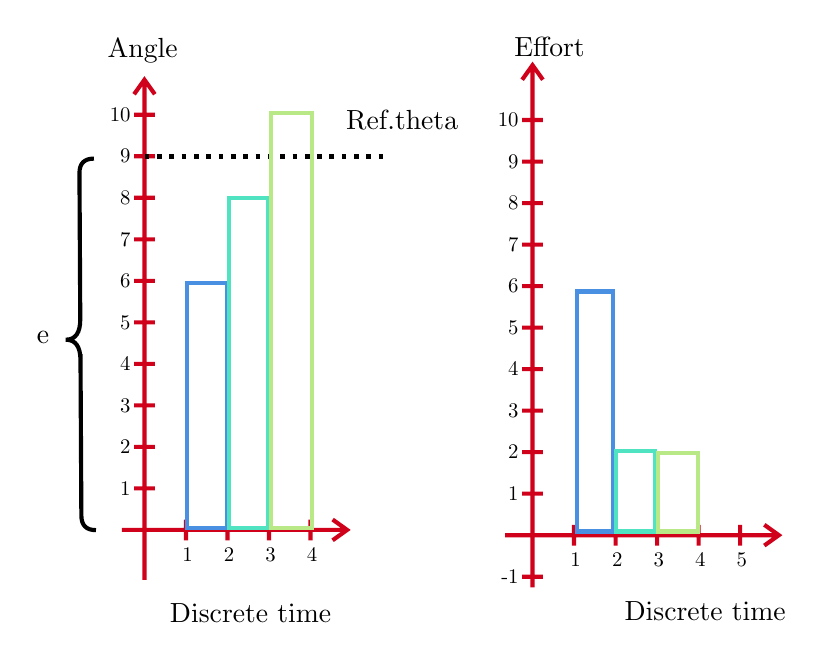
\begin{tikzpicture}[x=0.75pt,y=0.75pt,yscale=-1,xscale=1]
%uncomment if require: \path (0,530); %set diagram left start at 0, and has height of 530

%Shape: Axis 2D [id:dp9137510297707208] 
\draw [color={rgb, 255:red, 208; green, 2; blue, 27 }  ,draw opacity=1 ][line width=1.5]  (90,242.9) -- (198.5,242.9)(100.85,26) -- (100.85,267) (191.5,237.9) -- (198.5,242.9) -- (191.5,247.9) (95.85,33) -- (100.85,26) -- (105.85,33) (120.85,237.9) -- (120.85,247.9)(140.85,237.9) -- (140.85,247.9)(160.85,237.9) -- (160.85,247.9)(180.85,237.9) -- (180.85,247.9)(95.85,222.9) -- (105.85,222.9)(95.85,202.9) -- (105.85,202.9)(95.85,182.9) -- (105.85,182.9)(95.85,162.9) -- (105.85,162.9)(95.85,142.9) -- (105.85,142.9)(95.85,122.9) -- (105.85,122.9)(95.85,102.9) -- (105.85,102.9)(95.85,82.9) -- (105.85,82.9)(95.85,62.9) -- (105.85,62.9)(95.85,42.9) -- (105.85,42.9) ;
\draw   (127.85,254.9) node[anchor=east, scale=0.75]{1} (147.85,254.9) node[anchor=east, scale=0.75]{2} (167.85,254.9) node[anchor=east, scale=0.75]{3} (187.85,254.9) node[anchor=east, scale=0.75]{4} (97.85,222.9) node[anchor=east, scale=0.75]{1} (97.85,202.9) node[anchor=east, scale=0.75]{2} (97.85,182.9) node[anchor=east, scale=0.75]{3} (97.85,162.9) node[anchor=east, scale=0.75]{4} (97.85,142.9) node[anchor=east, scale=0.75]{5} (97.85,122.9) node[anchor=east, scale=0.75]{6} (97.85,102.9) node[anchor=east, scale=0.75]{7} (97.85,82.9) node[anchor=east, scale=0.75]{8} (97.85,62.9) node[anchor=east, scale=0.75]{9} (97.85,42.9) node[anchor=east, scale=0.75]{10} ;
%Straight Lines [id:da4351106715512081] 
\draw [line width=1.5]  [dash pattern={on 1.69pt off 2.76pt}]  (101,63) -- (218.5,63) ;


%Shape: Brace [id:dp994707289933978] 
\draw  [line width=1.5]  (76.5,64) .. controls (71.83,64.03) and (69.51,66.37) .. (69.54,71.04) -- (69.93,141.23) .. controls (69.97,147.9) and (67.66,151.24) .. (62.99,151.27) .. controls (67.66,151.24) and (70.01,154.56) .. (70.04,161.23)(70.03,158.23) -- (70.46,236.04) .. controls (70.49,240.71) and (72.83,243.03) .. (77.5,243) ;
%Shape: Rectangle [id:dp26090470643958286] 
\draw  [color={rgb, 255:red, 74; green, 144; blue, 226 }  ,draw opacity=1 ][line width=1.5]  (121.5,124) -- (140.5,124) -- (140.5,242) -- (121.5,242) -- cycle ;
%Shape: Rectangle [id:dp02841982011085853] 
\draw  [color={rgb, 255:red, 80; green, 227; blue, 194 }  ,draw opacity=1 ][line width=1.5]  (141.67,83) -- (160.5,83) -- (160.5,242) -- (141.67,242) -- cycle ;
%Shape: Rectangle [id:dp8528888145708966] 
\draw  [color={rgb, 255:red, 184; green, 233; blue, 134 }  ,draw opacity=1 ][line width=1.5]  (161.67,42) -- (181.67,42) -- (181.67,242) -- (161.67,242) -- cycle ;
%Shape: Axis 2D [id:dp5326952598948764] 
\draw [color={rgb, 255:red, 208; green, 2; blue, 27 }  ,draw opacity=1 ][line width=1.5]  (274.65,245.44) -- (406.5,245.44)(287.83,19) -- (287.83,270.6) (399.5,240.44) -- (406.5,245.44) -- (399.5,250.44) (282.83,26) -- (287.83,19) -- (292.83,26) (307.83,240.44) -- (307.83,250.44)(327.84,240.44) -- (327.84,250.44)(347.84,240.44) -- (347.84,250.44)(367.84,240.44) -- (367.84,250.44)(387.84,240.44) -- (387.84,250.44)(282.83,225.44) -- (292.83,225.44)(282.83,205.44) -- (292.83,205.44)(282.83,185.44) -- (292.83,185.44)(282.83,165.44) -- (292.83,165.44)(282.83,145.44) -- (292.83,145.44)(282.83,125.44) -- (292.83,125.44)(282.83,105.44) -- (292.83,105.44)(282.83,85.44) -- (292.83,85.44)(282.83,65.44) -- (292.83,65.44)(282.83,45.44) -- (292.83,45.44)(282.83,265.44) -- (292.83,265.44) ;
\draw   (314.83,257.44) node[anchor=east, scale=0.75]{1} (334.84,257.44) node[anchor=east, scale=0.75]{2} (354.84,257.44) node[anchor=east, scale=0.75]{3} (374.84,257.44) node[anchor=east, scale=0.75]{4} (394.84,257.44) node[anchor=east, scale=0.75]{5} (284.83,225.44) node[anchor=east, scale=0.75]{1} (284.83,205.44) node[anchor=east, scale=0.75]{2} (284.83,185.44) node[anchor=east, scale=0.75]{3} (284.83,165.44) node[anchor=east, scale=0.75]{4} (284.83,145.44) node[anchor=east, scale=0.75]{5} (284.83,125.44) node[anchor=east, scale=0.75]{6} (284.83,105.44) node[anchor=east, scale=0.75]{7} (284.83,85.44) node[anchor=east, scale=0.75]{8} (284.83,65.44) node[anchor=east, scale=0.75]{9} (284.83,45.44) node[anchor=east, scale=0.75]{10} (284.83,265.44) node[anchor=east, scale=0.75]{-1} ;
%Shape: Rectangle [id:dp37091810601651853] 
\draw  [color={rgb, 255:red, 74; green, 144; blue, 226 }  ,draw opacity=1 ][line width=1.5]  (309.42,128) -- (326.5,128) -- (326.5,243.67) -- (309.42,243.67) -- cycle ;
%Shape: Rectangle [id:dp5213748938493563] 
\draw  [color={rgb, 255:red, 80; green, 227; blue, 194 }  ,draw opacity=1 ][line width=1.5]  (328.08,205) -- (346.75,205) -- (346.75,243.67) -- (328.08,243.67) -- cycle ;
%Shape: Rectangle [id:dp3862836064219044] 
\draw  [color={rgb, 255:red, 184; green, 233; blue, 134 }  ,draw opacity=1 ][line width=1.5]  (348.08,206) -- (367.42,206) -- (367.42,243.67) -- (348.08,243.67) -- cycle ;

% Text Node
\draw (225,45.33) node  [align=left] {Ref.theta};
% Text Node
\draw (52,150) node  [align=left] {e};
% Text Node
\draw (100,12) node  [align=left] {Angle};
% Text Node
\draw (152,283) node  [align=left] {Discrete time};
% Text Node
\draw (296,10) node  [align=left] {Effort};
% Text Node
\draw (371,282) node  [align=left] {Discrete time};


\end{tikzpicture}
    \caption{A $K_D$ gain of 1 then only the rate of change in the error has and effect on the effort.}
    \label{fig:DGain}
\end{figure}

\paragraph{Discrete time} In the real world we live in a continues time domain, but computers works in discrete time domain. The discrete time is not measured in seconds, but rather in time frames.\\

On a note to a PID controller in theory, the perfect gains can be found, with the most suited rise time and settling time, but in practise this can be an expensive task. The expenses of the system can get high due to the need of a motor that is able to spin and stop at a rate that is suited for the PID controller, and sensors for the system needs to sense the changes within the system at the same rate.\\

\subsubsection{Dynamixel Servo PID}
In each Dynamixel servo there is an build in controller, that contains a feedback loop with an implemented PID controller with limiters to ensure that servos rotation velocity do not exceed a lower and an high threshold\cite{PIDmxx}. The feedback loop and the PID controller can be customised to fit the purpose of the objective.
\begin{figure}[H]
    \centering
    \includegraphics[width=\textwidth]{Figures/Technical_figures/PIDMX.PNG}
    \caption{Internal build in PID controller\cite{PIDmxx}}
    \label{fig:PIDMX}
\end{figure}

The servos positing and velocity is analysed through the use of an encoder, places on the gearing of the motor.  